


\pagebreak 
\section{Cyclical Wage Inequality}
\label{chap:Autostab_base}




\subsection{Cyclical Wage Dispersion} % widening earnings distribution cycle
In the baseline model all households are affected equally by changes in the aggregate wage rate. Additionally, the model assumes that a law of large numbers apply at the aggregate level such that firms hire the average worker. Households make no search decision and I rule out on the job search, so all households are subjected equally to job destruction and hiring. Resultingly, employment dynamics have no distributional effects either and business cycles are "neutral" per se. There exists a multitude of reasons why this is not necessarily the case. Agents in different parts of the earnings distribution might differ structurally in terms of age, education, geographical placement, gender and this might effect wages and employment status over the business cycle. The most obvious case occurs when agents have heterogeneous wages due to being employed in different sectors. \\

There are different ways to micro-found such mechanisms. One is on-the-job search as in \citet{moscarini2017job}. \citet{hubmer2018job} shows that a partial equilibrium model with on-the-job search generates a job-ladder type model. This type of model generates significantly more earnings risk in an endogenous way and fits the data better as opposed to the usual exogenous AR(1) processes for earnings risk with log-normal innovations. The addition of a search and matching labor market also aids in this regard, but only marginally through the job-finding rate. 



% Guvernen
\citet{guvenen2014nature} finds that income risk (as measured by the variance of household earnings) is acyclical. However, they document cyclical responses in the tails of the distribution. They find that the distribution of shocks become more left-skewed in recessions, implying that large positive shocks becomes less likely and adverse, negative shocks become more likely. This primarily related to within-group (earnings percentile) dispersion. For between-group dynamics, they find that earnings are most cyclical at the bottom and the absolute top of the earnings distribution. To this end, figure \ref{fig:Song_et_al} displays estimated elasticities of earnings to GDP from \citet{guvenen2017worker} as a measure of cyclicality by earnings percentiles. 

%31 Our model would feature an additional source of amplification if we introduced unequal income incidence, making
%income inequality countercyclical (see Bilbiie, Känzig and Surico 2019) - from micro jumps macro humps 

%It is worth noting that while Guvenen et al. (2014) find that the variance of household income is
%acyclical, they find that the left-skewness is countercyclical. Given our assumption of normally distributed
%income, skewness is constant in our model


%That is, during recessions, the
%upper end of the shock distribution collapses—large upward income movements become less likely—
%whereas the bottom end expands—large drops in income become more likely. Thus, while the dispersion
%of shocks does not increase, shocks become more left skewed and, hence, risky during recessions


\begin{figure}[H]
\makebox[\linewidth][c]{%
\centering
  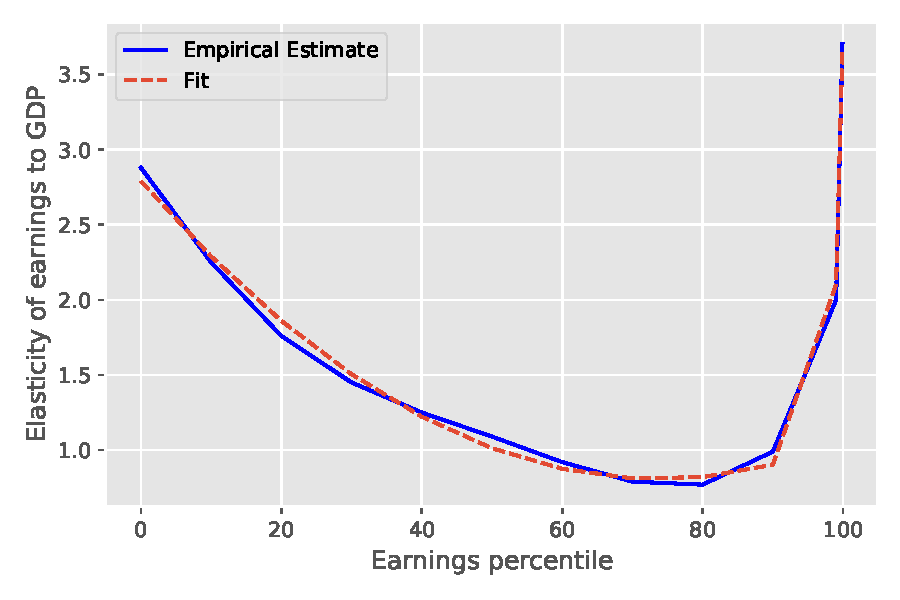
\includegraphics[width=.5\linewidth]{mainmatter/plots/cyclical_earnings/Song_earnings_cyclical.pdf} 
}
\caption{Estimated elasticity of earnings to GDP by percentile from \citet{guvenen2017worker}.}
\label{fig:Song_et_al}
 % {\scriptsize  Impulse responses to a negative productivity shock of 1\% with persistence 0.94 (half-life: 5 quarters). }
\end{figure}


Recent HANK models introduce endogenous, cyclical movements in the earnings distribution in ad-hoc manners. Analytical papers such as \citet{acharya2020understanding} assumes that the variance of labor supply depends on aggregate output. \citet{auclert2018inequality} does so by assuming that labor income contains a term $\gamma\left(e_{i,t},Y_{t}\right)$ that redistributes across the earnings distribution in response to cyclical changes as measured by $Y_t$.
Labor income in the two employment states are then given by $w_{t}\ell_{i,t}e_{i,t} \gamma\left(e_{i,t},Y_{t}\right)$ and $be_{i,t}\gamma\left(e_{i,t},Y_{t}\right)$. The function satisfies $\gamma\left(e_{i,t},Y^{ss}\right)=1$ such that there is no redistribution in steady-state. Furthermore $\gamma\left(e_{i,t},Y_{t}\right)=1$ for all $e_{i,t}$ such that the incidence function only redistributes across the earnings distribution but do not affect or alter aggregate income flows. 


Whether the incidence function introduces additional propagation or reduces volatility over the cycle is ambiguous. Households at the bottom of the earnings distribution tend to have higher MPCs whereas households at the top have low MPCs, and the effect on aggregate consumption hence depends on whether which of these effects dominate.  



%We introduce on-the-job search frictions in an otherwise standard monetary DSGE
%New-Keynesian model. Heterogeneity in productivity across jobs generates a job ladder. Firms Bertrand-compete for employed workers using the Sequential %Auctions protocol of Postel-Vinay and Robin (2002). Outside job offers to employed workers, when
%accepted, reallocate employment up the productivity ladder; when declined, because
%matched by the current employer, they raise production costs and, due to nominal
%price rigidities, compress mark-ups, building inflationary pressure. When employment
%is concentrated at the bottom of the job ladder, typically after recessions, the reallocation effect prevails, aggregate supply expands, moderating %arginal costs and inflation.
%As workers climb the job ladder, reducing slack in the employment pool, the inflation
%effect takes over. The model generates endogenous cyclical movements in the Neo
%Classical labor wedge and in the New Keynesian wage mark-up. The economy takes
%time to absorb cyclical misallocation and features propagation in the response of job
%creation, unemployment and wage inflation to aggregate shocks.